
\chapter{Theory of Units}\label{chap2} % \chapter II

\setcounter{section}{3}
\section{Units}\label{chap2:sec4}

\textbf{1.}~ Let\pageoriginale $\mathcal{J}$ be an order in the
quaternion algebra $Q/ k$; 
then a necessary and sufficient condition that an element
$\varepsilon$ in $\mathcal{J}$ be a unit in $\mathcal{J}$ is that
$n(\varepsilon)$ be a unit in $\mathscr{O}$. It is easy to see that
the units in $\mathcal{J}$ form a group which we denote by
$\mathscr{O}_\mathcal{J}$. In the case of definite algebras $Q/k$, we
have the following  
\setcounter{theorem}{0}
\begin{theorem}\label{chap1:sec4:thm1} % them 1
  {\em If $Q/k$ is definite, then $\mathscr{O}_\mathcal{J}$ is of finite order}.
\end{theorem}
 
\begin{proof}
  Let $\mathcal{J}= [L_1 \cdots L_4]$ and $\varepsilon= e_1 L_1 +
  \ldots + e_4 L_4$, a unit in $\mathcal{J}$. 
  $$
  n(\varepsilon) =e^2_1 n(L_1) + \cdots + e_1 e_2 t(L_1 \bar{L}_2)+ \cdots =1.
  $$
  $Q$ being definite, the quadratic form given by the norm is definite
  and consequently  the equation $n(\varepsilon)=1$ with real
  coefficients $e_1, \ldots,  e_4$ represent an ellipsoid in
  $R_4$. Hence there are only  a finite number of lattice points on
  this surface. In other words there are only a finite number of
  integral $e_1 \cdots e_4$ for which  $n(\varepsilon)=1$, i.e.,
  $\mathscr{O}_\mathcal{J}$ is of finite order. 
\end{proof} 

\begin{note}
  In fact, we have the converse part also to be true in this case,
  namely, if $Q$ is indefinite, $\mathscr{U}_\mathcal{J}$ is
  infinite. (We shall not give the proof here). 
\end{note}

We shall now consider unit groups of order of $Q/ k \cong
\mathfrak{M}_2(k)$. Let $\mathcal{J}$ be the maximal order
$\begin{pmatrix} \mathscr{O} & \mathscr{O} \\ \mathscr{O} &
  \mathscr{O} \end{pmatrix}$. Then the group of units $\mathscr{U}=
\Bigg\{ \begin{pmatrix} a & b \\ c & d \end{pmatrix}$, $a$, $b$, $c$, $d$ $\in
\mathscr{O} \text{ and } ad-bc= \pm, 1 \Bigg\}$ is simply the
unimodular group $\Gamma$ of\pageoriginale $(2,2)$ matrices and the subgroup
$\mathscr{U}_1$ of proper units of $\mathcal{J}$ (i.e., $ad-bc=1$) is
nothing but the modular group $\Gamma_1$, which is a normal subgroup
of $\Gamma$ of index $2$. 

We know that $\Gamma_1$ as a group acting on the upper half plane is
discontinuous and we have a fundamental domain (say) $D_1$. If
$\mathcal{J}_o$ is any  order $\subset \mathcal{J}$, then the group of
proper units of $\mathcal{J}_o$, say $\mathscr{U}_0 \subset
\mathscr{U}_1$. Consequently $\mathscr{U}_0$ as a group acting on the
upper half plane, is discontinuous and let $D_0$ be its fundamental
domain. 

Now, $\mathscr{U}_0 $ is of finite index in $\mathscr{U}$. Just as we
had in the $p$-adic case (\S \ref{chap1:sec3}, Proof of
lemma \ref{chap1:sec3:thm2:polem1}) we have a coset
decomposition  
$$
\mathscr{U}_1 = \bigcup^h_{i=1} \mathscr{U}_0 \varepsilon_i
$$

Then it can easily be-seen that $D_0$ can be taken to be
$\bigcup\limits_{i=1}^h \varepsilon_i D_1$;  $\varepsilon_i D_1$, the
image of $D_1$, by means of $\varepsilon_i$. 

We shall take up the remaining case, namely when $Q$ is indefinite and
also a division algebra. 

If $Q=[1, \omega, \Omega, \omega \Omega], \omega^2 = p, \Omega^2 =q,
(\omega \Omega)^2=- pq$, since $Q$ is indefinite, at least one of the
three $p,q, -pq$ is positive and we assume without loss of generality
that $p > 0$. 

Since $Q$ splits over $K \cong k(\sqrt{p})$, we have the following
isomorphism of $QK$ onto $\mathfrak{M}_2(K) \cong \mathfrak{M}_2
(k(\sqrt{p}))$. 
{\fontsize{10pt}{12pt}\selectfont
$$
1 \rightarrow 
\begin{pmatrix} 
  1 & 0 \\ 0 & 1
\end{pmatrix},
\omega \to 
\begin{pmatrix}
  \sqrt{p} & 0 \\
  0 & -\sqrt{p}
\end{pmatrix}, 
\Omega \to 
\begin{pmatrix}
  0 & 1 \\ q  & 0
\end{pmatrix}
\text{\ and\ } \omega \Omega \to 
\begin{pmatrix}
  o & \sqrt{p} \\
  -q \sqrt{p} & 0
\end{pmatrix}    
$$}\relax



Consequently, any element $\xi \in Q, \xi= X_1 + X_2 \omega + X_3
\Omega +  X_4 \omega \Omega$ has\pageoriginale the image
$\begin{pmatrix} X_1 + X_2 
  \sqrt{p} & X_3 + X_4 \sqrt {p}\\ q(X_3 - X_4 \sqrt{p}) & X_1 - X_2
  \sqrt{p}) \end{pmatrix}$, i. e., $\begin{pmatrix} \xi_1 & \xi_2 \\ q
  \bar{\xi}_2 & \bar{\xi}_1 \end{pmatrix}$ if $\xi _1 = X_1 + X_2
\sqrt{p}, \xi_2 = X_3 + X_4 \sqrt{p}; \xi_1,  \xi_2 \in k (\sqrt{p})$
and $\bar{\xi}_1,  \bar{\xi}_2$ denote the algebraic conjugates of
$\xi_1,  \xi_2 $ in $k (\sqrt{p})$.  

\textbf{2.}~ We wish to prove the existence of fundamental domains for unit
groups of orders in this case also and for the same, we require the
following two lemmas.  

Let $\mathcal{J}$ be an order and $\mathcal{J}= [ L_1 \cdots
  L_4]$. Consider all $\xi = L_1 x_1 + \cdots + L_4 x_4,  x_i $- real
and $n(\xi) = 1$. ($n (\xi)$ means simply the quadratic from with real
variables $x_1 \cdots x_4$). Then the set $M_c$ is defined as $\{ \xi
: |x_i | \leq c \} \cap \{ \xi : n (\xi) = 1\}$. In other words it is
the intersection of the cube $|x_i| \leq c$ in $R_4$ with the surface
$n(\xi) = 1$.  

\setcounter{Lemma}{0}
\begin{Lemma}\label{chap2:sec4:lem1} % lemma 1
  Let $\xi = L_1 x_1 + \cdots + L_4 x_4$, $x_i$ - real and $n(\xi) =
  1$. Then there exists only a finite number of units (say)
  $\varepsilon _1 \ldots \varepsilon_n$ so that if for any $\xi \in
  M_c,  \xi $ and $\varepsilon \xi \in M_c,  \varepsilon$, an unit of
  $\mathcal{J}$, then $\varepsilon$ is one of $\varepsilon_1 \ldots
  \varepsilon_n$. (This lemma is true even if $Q$ is not a division
  algebra ).  
\end{Lemma}

\begin{Lemma}\label{chap2:sec4:lem2} % lemma 2
  $Q/k$ is a division algebra and $\xi = \sum\limits_{j=1}^{4} L_j
  x_j,  x_j $- real and $n (\xi)=1$. Then there exists a constant $C$
  independent of $\xi$, and a unit $\varepsilon$ of $\mathcal{J}$,
  such that $\varepsilon \xi = \eta \in M_c$.  
\end{Lemma}

\setcounter{proofoflemma}{0}
\begin{proofoflemma}\label{chap2:sec4:polem1} % Proof of lemma 1
  Let $\eta = \varepsilon \xi = \sum\limits_{j=1}^{4} L_j y_j,
  \varepsilon $, a unit of $\mathcal{J}$. Then we have $\varepsilon =
  \eta \xi^{-1} = \eta.  \xi = L_1 e_1 + \cdots+ L_4 e_4$ (say) where
  $e_i \in \mathscr{O}$.  Further $e_i$ are bilinear forms in the
  coefficients of $\xi$ and\pageoriginale $\eta$. If $\xi$ and $\eta = \varepsilon
  \xi \in M_c$, then $|x_i | \leq c, |y_j| \leq c$ so that $|e_i| \leq
  c'$ ($c'$ depending on $c$ only ), $e_i$ being integers, there can be
  a finite number of them satisfying the above condition and hence our
  lemma.  
\end{proofoflemma}

\begin{proofoflemma}\label{chap2:sec4:polem2} % Proof of lemma 2
  Let $\beta = \alpha \xi,  \alpha \in \mathcal{J} = [ L_1 \ldots L_4
  ]$. If $\alpha = \sum\limits_{i=1}^{4} \alpha _i L_i$, then $\beta=
  \sum\limits_{i=1}^{4} \alpha_i L_i \xi$. But $L_i.  \xi =
  \sum\limits_{j=1}^{4} L_i L_j X_j = \sum\limits_{j, k}
  \lambda^{(k)}_{ij} X_j L_k$ if $L_i L_j = \sum\limits_{k=1}^{4}
  \lambda^{(k)}_{ij} L_k$.  
  $$
  \displaylines{\text{i. e.,}\hfill 
    L_i \xi = \sum_{k=1}^{4} c_{ik} L_k,  c_{ik} - ~\text{real}.\hfill } 
  $$
\end{proofoflemma}

Then we know that $|(c_{ik})| = (n(\xi))^2$. Hence $\beta =
\sum\limits_{i, k} a_i c_{ik} L_k = \sum\limits_{k=1}^{4} b_k L_k$ if
$b_k = \sum\limits_{i=1}^{4} a_i c_{ik}, b_k$ are linear forms in $a_1
\cdots a_4$ and their determinant $|c_{ik}| = n (\xi)^2 = 1$.  

Applying Minkowski's Theorem on linear forms to $b_k$, we can find
integral values for $a_1, \ldots,  a_4$ not all zero such that $|b_k|
\leq 1$, $k=1$ to $4$. Putting $\alpha = \sum\limits_{i=1}^{4} a_i L_i\,
(\alpha \in \mathcal{J})$ and $\beta = \alpha \xi$ we have since
$|b_k| \leq 1, n (\alpha) = n (\beta) < \gamma$, where $\gamma$ is a
constant. Further $a_1 \cdots a_4$ not all zero imply that $\alpha
\neq 0$ and hence $n(\alpha) \neq 0$ from the fact that $Q$ is a
division algebra.  

Now, $\alpha \in \mathcal{J}$ and $n( \alpha) < \gamma$ imply that
since there can exist only a finite number of integral ideals
$\alpha_1 \mathcal{J} \ldots \alpha_h \mathcal{J}$ with norms bounded
by $\gamma, \alpha \mathcal{J} = \alpha _j \mathcal{J}$, i, e.,
$\alpha = \alpha _j \varepsilon, \varepsilon$, a unit of
$\mathcal{J}$. Therefore $\beta = \alpha_j \varepsilon \xi$, i.e.,
$\alpha^{-1}_{j} \beta = \varepsilon \xi = \eta $ (say ). Since
coefficients of $\beta $ are bounded and since $\alpha_j$ come from a
finite set, the 
coefficients of\pageoriginale $\eta $ are bounded (say) are by $c$, and further
$n (\eta) = 1$. Hence $\eta \in M_c$ and thus Lemma
\ref{chap2:sec4:lem2} is proved.   
\begin{Lemma}\label{chap2:sec4:lem3} % lemma 3
  In Lemmas \ref{chap2:sec4:lem1} and \ref{chap2:sec4:lem2},  we can
  replace $L_1 \cdots L_4$ by any four 
  linearly independent elements $k_1,  \ldots k_4$ of $Q/ k$.  
\end{Lemma} 
 
 This follows from the fact that $[ L_1 \cdots L_4]$ and $k_1,
 \ldots,  k_4$ are connected by means of non-singular transformation
 and accordingly the proofs of Lemmas \ref{chap2:sec4:lem1} and
 \ref{chap2:sec4:lem2} go through except for
 the fact that the constant $c$ has to be replaced by another $c'$.  
  
Let $Q$ be an indefinite quaternion algebra over $k$. We shall take
for $k_1,  k_2,  k_3,  k_4$ the matrices $\begin{pmatrix}1 & 0 \\ 0 &
  0 \end{pmatrix}, \ldots, \begin{pmatrix} 0 & 0 \\ 0 &
  1 \end{pmatrix}$ respectively. (This is possible even if $Q$ be a
division algebra, because it splits over $K \simeq k (\sqrt{p})\, (p >
0)$).  
 
Let $\mathscr{H}$ be the space of all $(2, 2)$ real matrices with
determinant $1$. In particular $\mathscr{H}$ contains all elements
$\xi$ of $Q$ with $n (\xi) = 1$. We now map $\mathscr{H}$ onto the
complex upper half plane $S$.  

If $\xi = \begin{pmatrix} x_{11} & x_{12} \\ x_{21} &
  x_{22}\end{pmatrix}$ with $x_{11} x_{22} - x_{12} x_{21} = 1$,
define the mapping $\varphi : \mathscr{H} \to S$ by $\varphi (\xi) =
\xi(i) = \dfrac{x_{11} i + x_{12}}{x_{21 } i + x_{22}}$.  

 Since $\im  (\xi(i)) = \dfrac{1}{x^{2}_{21} + x^{2}_{22}},
 \varphi(\xi)$ is onto; for
\begin{equation*}
  \begin{pmatrix}
    a / \sqrt{b} & \sqrt{b} \\ 1 / -\sqrt{b} & 0
  \end{pmatrix}
  (i) = a + ib. 
\end{equation*}

\begin{Lemma}\label{chap2:sec4:lem4} %lemma 4
  The set $M_c = \bigg\{ \begin{pmatrix} x_{11} & x_{12} \\ x_{21} &
    x_{22}\end{pmatrix}$ $x_{ij}$ real and $|x_{ij}| \leq c$, $x_{11}
    x_{22}- x_{12} x_{21}= 1 \bigg \} \subset \mathscr{H}$\pageoriginale is mapped
    by $\varphi$ onto finite part of the upper half plane $S$ and
    conversely, any domain in $S$ consisting of $\bigg\{ \tau : |\tau|
    < C_1, \im  \tau > c_2 \bigg \}$ has an inverse contained in $M_c$
    for some $c$.  
 \end{Lemma}  

\begin{proof}
  Now $|x_{ij}| < c \Longrightarrow |x_{11} i + x_{12}| < 2c $ and
  $|x_{12} i + x_{22}|< 2c$. Further $0 \leq d < |x_{21} i + x_{22} |<
  2 ~ c$, for 
  $$
  \big| (x_{22} - x_{21} i ) (x_{11} i + x_{12}) \big| = \big|(x_{22}
  x_{12} + x_{11} x_{21}) + i \big| \leq C' 
  $$
  implies that if $\big|x_{21} i + x_{22}\big|$ were arbitrarily
  small, $|x_{11} i + x_{12}|$ would increase arbitrarily, which is
  not true.  
\end{proof} 

Hence $\im  (\xi (i)) = \dfrac{1}{\big|(x_{21} i + x_{22})\big|^2} >
\dfrac{1}{c^2}$ so that $M_c$ is mapped onto a finite part of the
upper half plane. Conversely if $\tau = \dfrac{x_{11} i +
  x_{12}}{x_{21} i + x_{22}}$ is such that $ x_{11} x_{22} - x_{12}
x_{21} =1$, $|\tau| < c_1$ and $\im  \tau > c_2$, then
$\dfrac{1}{x^{2}_{21}+ x^{2}_{22}} > c_2 \Longrightarrow
\big|x_{21}\big| < c_3,  \big| x_{22}\big| < c_3$. Further
$\dfrac{x^{2}_{11} + x^{2}_{12}}{x^{2}_{21} + x^{2}_{22}} < c^{2}_{1}
\Longrightarrow x^{2}_{11} + x^{2}_{12} < \dfrac{c_1^2}{c_2}
\Longrightarrow \big|x_{11} 
\big| < c_4,  \big|x_{12}\big| < c_4$. Choosing $c = \max (c_3,
c_4)$, it follows that $\big|x_{ij}| < c,  i,  j = 1, 2$. From here
onwards, we shall use the notation $M_c$ for the image of $M_c$ by
means of $\varphi$, in the upper half plane $S$. If $\xi,  \eta \in
\mathscr{H}$, then we shall prove that $\varphi (\eta \xi) - (\eta
\xi) (i) = \eta (\xi (i))$. For, let $\xi = \begin{pmatrix} x_{11}
  &x_{12}\\ x_{21} & x_{22} \end{pmatrix}$ and $\eta = \begin{pmatrix}
  y_{11}& y_{12} \\ y_{21} & y_{22}\end{pmatrix}$. Then  
\begin{align*}
 (\eta \xi ) (i) & = \frac{(y_{11} x_{11} + y_{12} x_{21}) i + (y_{11}
  x_{12} + y_{12} x_{22})}{(y_{21}x_{11} + y_{22} x_{21}) i + (y_{21}
  x_{12} + y_{22} x_{22})} \\
 & = \frac{y_{11} \left(\frac{x_{11} i + x_{12}}{x_{21} i + x_{22}}\right) +
  y_{12}}{y_{21}\left(\frac{x_{11}i + x_{12}}{x_{21} i + x_{22}}\right) +
  y_{22}} = \frac{y_{11} \xi (i) + y_{12}}{y_{21} \xi (i) + y_{22}}
\end{align*}
$\xi (i)$\pageoriginale being a point of the upper half plane $S$ and since
$\mathscr{H}$ acts as a group of mapping on $S, \dfrac{y_{11} \xi (i)
  + y_{12}}{y_{21} \xi (i)+ y_{22}} = \eta (\xi (i))$. Thus we have the
important passage from a mapping of $\mathscr{H} : \xi \to \eta \xi$
to a mapping of the upper half plane: $\xi (i) \to \eta (\xi (i))$ by
means of $\varphi$. This enables us to carry over our lemmas for
$\mathscr{H}$ to those for $S$, as follows: 

\begin{lem}\label{chap2:sec4:lem'1} % lemma 1'
  Given a finite domain $M_c$ in $S$, there exists only a finite
  number of units $\varepsilon_1,  \ldots,  \varepsilon_n$ in order
  $\mathcal{J}$ of $Q$ such that if $\tau$ and $\varepsilon (\tau)$
  are in $M_c$($\varepsilon$, a unit of $\mathcal{J}$) then
  $\varepsilon$ is one of $\varepsilon _1 \cdots \varepsilon_n$.  
\end{lem}

\begin{lem}\label{chap2:sec4:lem'2}  % lemma 2'
  If $Q$ is a division algebra, then there exists an $M_c$ in $S$ such
  that for any $\tau \in S$, we can find at least one unit
  $\varepsilon$ of $\mathcal{J}$ such that $\varepsilon (\tau) \in M_c
  $.  
\end{lem}

 If $\mathscr{H}$ is the group of proper units of an order
 $\mathcal{J}$ in $Q$ $\mathscr{O} \subset \mathscr{H}$and using the
 lemma \ref{chap2:sec4:lem'1}$'$ we shall construct a fundamental
 domain for $\mathscr{O}$ in 
 $S$. We will further prove using lemma \ref{chap2:sec4:lem'2}$'$ that
 $D$is bounded in the 
 case of a division algebra $Q$ and in general $D$ has only a finite
 number of neighbours.  
 
\begin{note}
  One may also proceed alternatively for proving the existence of a
  fundamental domain for $\mathscr{O}$ in $S$, as follows: If
  $\mathcal{L}$ is the inverse image of the point $i$, by means of
  $\varphi$, in $\mathscr{H}$, then $\bar{\mathcal{L}}$ is the proper
  orthogonal group and consequently a compact subgroup of the
  topological group $\mathscr{H}$. Then it can be proved that the
  mapping $f: \dfrac{\mathscr{H}}{\mathcal{L}} \to S$ defined by $f
  (\xi \mathcal{L}) = \varphi (\xi) = \xi (i)$ is one-one open\pageoriginale and
  continuous. The latter part follows from the fact that $\varphi$ is
  open and continuous. From Lemma \ref{chap2:sec4:lem'1}$'$, we obtain $\mathscr{O}$ is
  discrete in $\mathscr{H}$ and $\bar{\mathcal{L}}$ being compact, it
  follows that $\mathscr{O}$ has a discontinuous representation in
  $\dfrac{\mathscr{H}}{\mathcal{L}}. \dfrac{\mathscr{H}}{\mathcal{L}}$
  being homeomorphic to $S$, this implies that $\mathscr{O}$ acts as a
  discontinuous group of mapping on the upper half plane $S$ and thus
  we have the existence of a fundamental domain for $\mathscr{O}$ in
  $S$.  
\end{note}
   
We shall now sketch a method of constructing of a fundamental domain
for the group $\mathscr{O}$ in $S$. For the same we consider the upper
half plane $S$ as a metric space with the hyperbolic metric $d$,
i.e.,  $d(x, y)$ is invariant under the group of hyperbolic motions.  

Choose a point $\tau$ in $S$, which is not a fixed point for any $\varepsilon
\neq 1 (\varepsilon \in \mathscr{O})$. Such a $\tau$ exists, for if
not, then for $\tau \in S$ there would exist an $\varepsilon \in
\mathscr{O}$ such that $\varepsilon (\tau) = \tau$. If $\tau \in M_c$,
then $\varepsilon (\tau) = \tau \in M_c$. But such $\epsilon -s$
are infinite in number, a contradiction to Lemma \ref{chap2:sec4:lem1}.  

Consider $\tau $ and $\varepsilon (\tau),  \varepsilon \neq 1,
\varepsilon \in \mathscr{O}$. Since $\tau \neq \varepsilon (\tau) $,
we can draw the perpendicular bisector of the hyperbolic line joining
$\tau $ and $\varepsilon (\tau)$. Then the hyperbolic plane $S$ is
divided into two half -planes, one consisting of points nearer to
$\tau$ than $\varepsilon (\tau)$, the other vice-versa. Carrying out a
similar construction for all $\varepsilon (\neq 1)$ of $\mathscr{O}$,
we finally obtain a domain $D$, which is the intersection of all open
half planes containing the point $\tau$. In other words\pageoriginale $D$ consists
of points which are nearer to $\tau$ than to any other $\varepsilon
(\tau)$. That $D$ is non-empty follows from Lemma \ref{chap2:sec4:lem'1}$'$.  We shall prove
now that $D$ is a fundamental domain (except for some boundary points)
for $\mathscr{O}$ in $S$. Accordingly, we shall verify the following: 

\begin{figure}[H]
\centerline{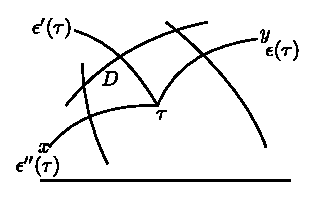
\includegraphics{vol9-figures/fig9-1.eps}}
\end{figure}
\begin{enumerate}[i)]
\item $D \cap \varepsilon D = (\phi)$ for every $\varepsilon (\neq 1)
  \in \mathscr{O}$. ($\varepsilon D$ denotes the image of $D$ by means
  of the transformation $\varepsilon$).  
\item $\bigcup\limits_{\varepsilon \in \mathscr{O}} \overline{\varepsilon D} = S$. 
\end{enumerate} 
 
\begin{proof}
  \begin{enumerate}[i)]
  \item If $D \cap \varepsilon D \neq (\phi)$ for some $\varepsilon$,
    there exists a $\sigma \in D \cap \varepsilon D$ so that $\sigma$
    and $\varepsilon ^{-1} (\sigma) \in D$. Since $\varepsilon$
    preserves the hyperbolic distance, we have 
    $$
    \displaylines{\hfill 
    d (\tau,  \varepsilon^{-1} (\sigma)) < d (\varepsilon ^{-1}
    (\tau), \varepsilon ^{-1} (\sigma)) = d (\tau,  \sigma) \hfill \cr
    \text{and}\hfill  
    d (\tau,  \sigma) < d (\varepsilon (\tau),  \sigma) = d (\tau,
    \varepsilon ^{-1} (\sigma))\hfill  }
    $$
    which are contradictory. 
  \item Let $\rho$ be any point of $S$. Then there exists at least one
    $\varepsilon (\tau)$ which is nearer to $\rho$ than $\varepsilon '
    (\tau), \varepsilon' \neq \varepsilon$. For, if not, in a
    neighbourhood of $\rho$ we would have an infinity of $\varepsilon
    (\tau)$ which contradicts Lemma
    \ref{chap2:sec4:lem'1}$'$. Therefore $\rho$ lies in 
    $\varepsilon D$. If $\varepsilon (\tau)$ and $\eta (\tau)$ are
    equidistant from $\rho$ and are nearer to $\rho$ than any other
    $\varepsilon' (\tau)\, (\varepsilon \neq \varepsilon,  \eta)$ is
    from $\rho$, then $\rho$ lies on the boundary of $\varepsilon D$
    and $\eta D$. Thus, we have the second assertion.  
  \end{enumerate}
\end{proof}

%%% repeated theorem 1 in this section  so (refer for thmm1)

\setcounter{theorem}{0}
\begin{theorem}\label{chap2:sec4:thmm1} % theorem 1
  In case $Q$ is a division algebra, the fundamental domain $D$
    is bounded 
\end{theorem}

\begin{proof}
  If not, there will be a boundary point $\tau$ of $D$ on the real
  line\pageoriginale ($\tau$ can be the point at $\infty$ as
  well). Let $\{\tau_ i
  \}$ be a sequence of elements of $D$ having $\tau$ as a limit point
  and choose a subsequence $\{\tau_{n_i}\}$ converging to $\tau$. Then,
  by Lemma \ref{chap2:sec4:lem'2}$'$, there exists an $M_c$ for which
  $\varepsilon _{n_i} 
  (\tau_{n_i}) \in M_c ; \varepsilon _{n_i} \in \mathscr{O}$. Further
  $\varepsilon _{n_i} (\tau_{n_i}) \in \varepsilon _{n_i} D$ so that
  $\varepsilon_{n_i} (\tau_{n_i}) \in M_c \cap \varepsilon _{n_i}
  D$. But $M_c \cap \varepsilon D$ is non-empty only for a finite
  number of $\varepsilon \in \mathscr{O}$ from Lemma \ref{chap2:sec4:lem'1}$'$, so that
  $\varepsilon_{n_i} (\tau_{n_i}) \in M_c \cap \varepsilon D$ for $n_i
  \geq n_o$ (say), for a fixed $\varepsilon$.  
\end{proof} 

Now, $\varepsilon _{n_i} (\tau_{n_i}) = \varepsilon (\lambda_i),
\lambda_i \in D \Longrightarrow \tau_{n_i} = \lambda _i$ since no two
distinct points of $D$ are equivalent. Therefore $\varepsilon _{n_i} =
\varepsilon$.  

 Since $\tau_{n_i} \to \tau$, $\varepsilon (\tau_{ni}) \to \varepsilon
 (\tau)$. But $\varepsilon (\tau _{n_i}) \in M_c$ so that $\varepsilon
 (\tau) \in M_c$ for $M_c$ is closed. This is contradictory to Lemma
 \ref{chap2:sec4:lem4}
 for $\varepsilon $ is a real transformation and $\tau$ is a real
 point.  
 
 \begin{theorem}\label{chap2:sec4:thmm2} % theorem 2
   {\em $D$ has only a finite number of neighbours in either case
     whether $Q$ is a matrix or division algebra. } 
 \end{theorem} 

From this it would follow that there are only a finite number of
$\varepsilon_i D$, $\varepsilon_i \in \mathscr{O}$ which have boundary
points in common with $D$. In other words there exists a fundamental
polygon $D$ with a finite number of sides.  

\begin{proof}
  Suppose $D$ does not have a finite number of neighbours. Then it has
  an infinite number, i. e.,  $D$ has an infinite number of sides $\{
  c_i \}$ (say). Let $\varepsilon _i (\tau)$ be the reflections of
  $\tau$ at these $c_i$ respectively. Then we have to distinguish two
  cases.  
\end{proof}

\begin{enumerate}[(i)]
\item $\big\{ \varepsilon_i (\tau)\big\}$ have a finite limit point $\tau$ (say)
\item $\big\{ \varepsilon _i (\tau)\big\}$ have a limit point at
  infinity (i. e.,  real).  
\end{enumerate}

In\pageoriginale case (i) we choose a subsequence $\big\{ \varepsilon _{n_i}
(\tau)\big\}$ (say) which converges to $\tau$. Then we may select a
neighbourhood $N$ of $\tau$ contained in some $M_c$. By the nature of
$\tau$, there exists an infinity of $\varepsilon _{n_i}	 (\tau)$
inside $N$ and hence in $M_c$, which is contradictory to Lemma
\ref{chap2:sec4:lem'1}$'$.  

In case (ii), we easily see that this arises only if $Q$ is a matrix
algebra, since $D$ is bounded otherwise, by $(b)$. Then $\mathscr{U}$
is a subgroup of the modular group $\Gamma_1$, so that if the coset
decomposition given by $\Gamma _1 = \sum\limits_{i=1}^{n}
\mathscr{U}. \varepsilon_i$ we may get a fundamental domain for
$\mathscr{U}$ as $F = \sum\limits_{i=1}^{n} \varepsilon_i D_1,  D_1$
being a fundamental domain for the modular group $\Gamma_1$. $D$ and
$F$ are topologically equivalent and we know that $F$ has only a
finite number of sides and in fact only a finite number (say $n$) of
real boundary points or parabolic cusps (a parabolic cusp is a fixed
point of infinite order), since $D_1 $ has $\infty$ as the only
parabolic cusp.  

\section{Topological Properties of Units}\label{chap2:sec5} %section 5

\textbf{3.}~ We have already seen that the fundamental domain $D$ has only a
finite number of neighbours $\varepsilon_1 D_1,  \ldots,  \varepsilon
_n D$ say. In this connection we have the  
 
\setcounter{theorem}{0}
\begin{theorem}\label{chap2:sec5:thm1} % theorem 1
  The units $\varepsilon_1, \ldots, \varepsilon _n$ generate the
  whole group $\mathscr{O}$.  
\end{theorem}

\begin{proof}
  Let $P$ be a point of $D$, and $Q$ a point of $\varepsilon D$. Join
  $P$ and $Q$ by an arc. This are is contained in $M_c$ for some $c$,
  and $M_c$ intersects only finite number of $\eta D' -s, \eta \in
  \mathscr{U}$, so that the are $PQ$ is covered by a finite number of
  the $\eta D' s$. Then the neighbours of any $\eta D$ are given by
  $\eta \varepsilon _i D, i = 1, \ldots,  n$.  
\end{proof}

We\pageoriginale can go from $D$ to $\varepsilon D$ as follows:
$$
D, \varepsilon_{i_1} D,  \varepsilon_{i_1}. \varepsilon_{i_2} D,
\ldots,  \varepsilon_{i_1}. \varepsilon_{i_2} \cdots \varepsilon
_{i_k} D = \varepsilon D,  
$$
where $i_1, \ldots,  i_k$ lie between $1$ and $n$. This means
$\varepsilon = \varepsilon_{i_1} \cdots \varepsilon_{i_k}$. (It may be
remarked here that there exist certain relations between $\varepsilon
_1 \ldots,  \varepsilon_n$ which we will later obtain explicitly).  
\begin{enumerate}[(i)]
\item In the case that $Q$ is a division algebra the fundamental
  domain $D$ is bounded, and by identifying the pairs of equivalent
  sides we obtain a closed surface which we denote by
  $S_{\mathcal{J}}$. This surface can also be seen to be the same as the
  upper half plane modulo $\mathscr{O}$, i, e,.  $\mathscr{H}/
  \mathcal{L}$ modulo $\mathscr{O}$ which is the same as the space of
  double cosets $\mathscr{U} \xi \mathcal{L}$. It can also be seen that
  $S$ is an infinite sheeted covering surface of $S_{\mathcal{J}}$ 
  
\item In the case when $\Omega$ is a matrix algebra, we have at most
  a finite number of parabolic cusps, and the surface $S_{\mathcal{J}}$
  is obtained by identification of pairs of equivalent sides together
  with the adjunction of these cusps.  

\item $S_{\mathcal{J}}$ as a manifold is orientable. 

  This follows from the fact that the $\varepsilon' s$ considered as
  hyperbolic motions have positive determinant.  
  
\item \textit{Canonical form for the surface}$S_{\mathcal{J}}$

  In the fundamental domain $D$ is denoted by $a_1 \cdots a_n$ where
  $a_i$ are the sides, then we wish to obtain this in the canonical from
  $a_1 c_1 c^{-1}_1 b_1 c_2 c_2^{-1} a^{-1}_1 \cdots b^{-1}_1$ $\cdots
  c_k c_k^{-1} \cdots 
  a_g b^{-1}_{g}$ where $a^{-1}_{1}$ is the side equivalent to $a_1$
  with the opposite orientation.  
\end{enumerate}

\begin{figure}[H]
\centerline{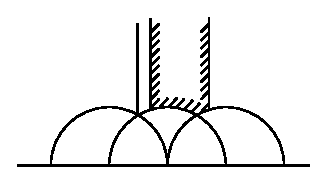
\includegraphics{vol9-figures/fig9-2.eps}}
\end{figure}
Figure a fundamental domain for the whole modular group in
  canonical form.

(There\pageoriginale may be more than one pair $c_1 c^{-1}_{1}$ between $a_1,  b_1$
and similarly at other places also). The surface obtained from this
reduced from is then called the canonical form for $S_{\mathcal{J}}$ 

The canonical from is obtained in two steps. 

\begin{enumerate}[(i)]
\item Reduction of \textit{elliptic vertices}. (i, e,.  the vertices
  which are fixed points of elliptic transformations).  
  
  Let $\tau $ be a vertex which is a fixed point, i. e.,  $\tau$ is
  the intersection of a pair of equivalent sides, say $c_1$ and
  $\varepsilon c_1$. We have the following two possibilities in the
  orientation of the sides.  
  
\begin{figure}[H]
\centerline{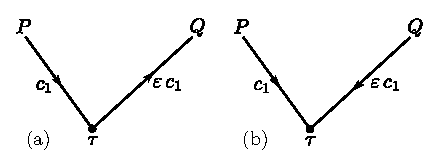
\includegraphics{vol9-figures/fig9-3.eps}}
\end{figure}

  Case $(a)$ is ruled out since the orientation of $\varepsilon c_1$
  induced by the orientation of $c_1$ would be opposite to that already
  present in $\varepsilon c_1$  
  
  We have then only the case $(b)$, and in this case we may consider
  $c_1 (\varepsilon c)^{-1}$ as an inseparable unit.  

\item Having dispensed with the case of elliptic vertices we now
  consider the polygon $D$ as one without fixed points. We now employ
  the classical procedure to obtain canonical form $a_1 b_1 a^{-1}_1
  b^{-1}_{1} \cdots a_g$ $b_g a^{-1}_{g} b^{-1}_g$. [For this see
    C. L. Siegel, Ausgewahlte Fragen der Funktionentheorie,  $I$
    (G\"ottingen). Pages 106 - 110, or Nevanlinna, ``
    Uniformisierung'', Chapter 7 \S 3].  
\end{enumerate}

However,\pageoriginale in our case, there do not exist free sides even in
the case of a matrix algebra.  

Combining both (i) and (ii), the required canonical form is obtained. 

We now have the 
\begin{theorem}\label{chap2:sec5:thm2} % them 2
  If $\varepsilon_a$ is the transformation which takes a to the
    side $a^{-1} (\varepsilon_a \in \mathscr{U})$, we have the
    following relations: 
  $$
  I \,\varepsilon_{b_g} \varepsilon^{-1}_{a_g} \varepsilon_{d_g}^{-1}
  \varepsilon_{a_g} \cdots \varepsilon_{b_1} \varepsilon^{-1}_{a_1}
  \varepsilon_{b_1} \varepsilon_{a_1} \cdot \eta_{c_k} \cdots
  \eta_{c_1} = 1; 
  $$
  and $\eta^{n_i}_{c_i} = 1$ for all $i$. 
\end{theorem}

$II (a)$ ~If $Q$ is a division algebra, and if $\tau$ is a parabolic
vertex, or cusp and if $\varepsilon_{\tau} (\tau) =\tau$, then
$\varepsilon_{\tau}$ is of infinite order. Here $\eta_{c_i}=
B^{-1}_{i} \varepsilon_{c_i} B_i$ and $B'_i  s$ are products of the
$\varepsilon'_a$ and $\varepsilon'_b  s$.  

\begin{proof}
To prove I we split it into two cases:

Let no fixed points exists between $P_1$ and $P_5$. Consequently we
have the following relations: 
\begin{align*}
  \varepsilon_{a_1} (P_1)  = P_4, \varepsilon_{a_1} (P_2) &= P_3, \\
  \varepsilon_{b_1} (P_3)  = p_4,  \varepsilon_{b_1} (P_2) & = P_5, \\
  \text{i, e,.}  \hspace{2cm}\varepsilon^{-1}_{a_1}.  \varepsilon_{b_1}^{-1}
  \varepsilon_{a_1}(P_1) & = P_2\hspace{1cm}\\  
  \text{and hence}\qquad \varepsilon_{b_1}.
  \varepsilon^{-1}_{a_1} \varepsilon_{b_1}^{-1} 
  \varepsilon_{a_1} (P_1) & = P_5.
\end{align*}

  \begin{figure}[H]
    \centerline{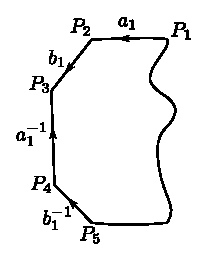
\includegraphics{vol9-figures/fig9-4.eps}}
  \end{figure}

Assuming that there are no fixed points, and proceeding as above, we obtain
$$
\varepsilon_{b_g} \varepsilon_{a_g}^{-1}
\varepsilon_{b_g}^{-1}\varepsilon_{a_g} \cdots 
\varepsilon_{b_1} \varepsilon_{a_1}^{-1} \varepsilon_{b_1}^{-1}
\varepsilon_{a_1} (P_1)= P_1,  
$$
and\pageoriginale since $P_1$ is not a fixed point, we have
$$
\varepsilon_{b_g}\varepsilon_{a_g}^{-1} \varepsilon_{b_g}^{-1}
\varepsilon_{a_g} \cdots \varepsilon_{b_1}\varepsilon_{a_1}^{-1}
\varepsilon_{b_1}^{-1} \varepsilon_{a_1} = 1.  
$$

(ii)~ In the case that there exist elliptic vertices, we may suppose,
for example, that one such lies between $a_1$ and $b_1$. In this case
we have  
\begin{align*}
  \varepsilon_{a_1} (P_1) & = P_6, \quad \varepsilon_{a_1} (P_2) = P_5, \\
  \varepsilon_{c_1} (P_3) & = P_3, \quad \varepsilon_{c_1} (P_2) = P_4, \\
  \varepsilon_{b_1} (P_4) & = P_7, \quad \varepsilon_{b_1} (P_5) = P_6, \\ 
  \text{i.e.,}  \qquad \varepsilon_{b_1} \varepsilon_{c_1} & \varepsilon_{a_1}^{-1}
\varepsilon_{b_1}^{-1} \varepsilon_{a_1} (P_1) = P_7.  
\end{align*}

  \begin{figure}[H]
    \centerline{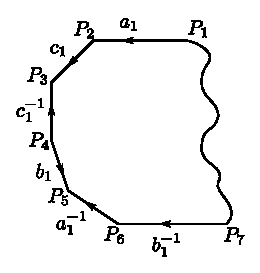
\includegraphics{vol9-figures/fig9-5.eps}}
  \end{figure}

\end{proof}

Proceeding in this manner, we obtain
$$
\varepsilon_{b_g}
\varepsilon_{a_g}^{-1}\varepsilon_{b_g}^{-1}\varepsilon_{a_g}\cdots
\varepsilon_{b_k}\varepsilon_{c_k} \varepsilon_{a_k}^{-1}
\varepsilon_{a_k}^{-1} \varepsilon_{a_k} \cdots
\varepsilon_{b_1}. \varepsilon_{c_1}
\varepsilon_{a_1}^{-1}\varepsilon_{b_1}^{-1} \varepsilon_{a_1} =1.  
$$

With an obvious notation, we write the above equation in the form 
$$
A_{k+1} \varepsilon_{c_k} A_k \varepsilon_{c_{ k-1}} \cdots A_2
\varepsilon_{c_1} A_1 = 1.  
$$

We may rewrite this as follows:  
$$
A_{k+1} \cdot A_k \cdot \cdot A_1 (A_k \cdot \cdot A_1 )^{-1}
\varepsilon_{c_k} (A_k \cdot \cdot A_1) \cdot \cdot (A_2 A_1)^{-1}
\varepsilon_{c_2} (A_2 A_1)\cdot A_1 ^{-1}\varepsilon_{c_1} A_1 = 1.  
$$

Let $\eta_{c_i} = (A_i A_{i-1} \cdot \cdot A_1 )^{-1}
\varepsilon_{c_i}(A_i \cdot \cdot A_1)$, then the above relation can be
written in the form 
$$ 
\varepsilon_{b_g}\varepsilon_{a_g}^{-1}\varepsilon_{b_g}^{-1}\varepsilon_{a_g}
\dot \dot \varepsilon_{b_1}
\varepsilon_{a_1}^{-1}\varepsilon_{b_1}^{-1} \varepsilon_{a_1}
\eta_{c_k} \cdots \eta_{c_1} = 1.  
$$

 Let now the transformations $\varepsilon_{c_1},  \ldots,
 \varepsilon_{c_k}$ have $\tau_1,  \ldots,  \tau_k$ as their fixed
 points (we suppose that no $\tau_i$ is a cusp ). We can then find a
 neighbourhood of $\tau_i$ which is contained in some $M_c$. If now
 $\varepsilon _{c_i}$ is not of finite order, then $\varepsilon_{c_i},
 \varepsilon_{c_i}^{2}, \ldots,  $ are all distinct, and\pageoriginale
 $\varepsilon_{c_i}^{n} (\tau_i) = \tau_i $ for all $n$, and this
 contradicts Lemma \ref{chap2:sec4:lem1}. Hence $\varepsilon_{c_i}$ is
 of finite order $n_i$, and then we have  
$$
\varepsilon_{c_1}^{n_1} = \cdots = \varepsilon_{c_k}^{n_k}= 1. 
$$

From this equation it follows that $\eta _{c_1}^{n_1} = \cdots = \eta
_{c_k}^{n_k} = 1$. (b) Since the above argument breaks down in
the case of a parabolic vertex or a rational fixed point $\tau_o,
(\tau_o \neq 0,  \infty)$, we cannot conclude that $\varepsilon_c$
which fixes $\tau_o$ is of finite order. We now prove that it is
necessarily of infinite order.  

Since $\tau_o \neq \infty $, we obtain a transformation $\eta$ such
that $\eta (\tau_o) = \infty$. We only have to take $\eta
= \begin{pmatrix} -1 / \tau_o & 0 \\ 1 & -\tau_o \end{pmatrix}$.  

Then $\eta \varepsilon_c \eta^{-1} = \varepsilon'_c$ has $\eta
(\tau_o) = \infty$ as fixed point $\varepsilon'_c$ must then
necessarily have the form $\varepsilon'_c = \begin{pmatrix} a & b \\ 0
  & d \end{pmatrix}$, and on multiplication by $\begin{pmatrix} \pm 1
  & 0 \\ 0 & \pm 1 \end{pmatrix}$, we may assume that $a > 0,  d > 0$.  

Further $\varepsilon'_c \neq 1$, for otherwise $\varepsilon_c =
1$. Suppose $\varepsilon_c ^n = 1$. Then $\varepsilon'^{n}_{c} =
1= \begin{pmatrix}1 & 0 \\ 0 & 1 \end{pmatrix} = \begin{pmatrix}a^n &
  B_n \\ 0 & d^n \end{pmatrix}$, i. e.,  $a^n = d^n = 1$, or $a= d=
1$, for $a> 0$ and $d > 0$. Now $B_n = nb = 0$ implies that $b= 0$, or
$\varepsilon'_c = 1$ which is a contradiction.  

\begin{theorem}\label{chap2:sec5:thm3} % theorem 3
  \begin{enumerate}[\rm (1)]
  \item For any two $ \varepsilon_{c_i}, \varepsilon_{cj},
    \eta^{-1} \varepsilon_{c_i}.\eta \neq \varepsilon_{cj}$ for any
    $\eta$.  
  \item If $\varepsilon$ has the fixed point $\tau$, then there
    exists an $\eta $ such that  
    $$
    \eta^{-1} \varepsilon \eta = \varepsilon_{c_i} ~\text{for some }~ i. 
    $$
  \end{enumerate}
\end{theorem}

\begin{proof}
  \begin{enumerate}
  \item $\eta^{-1} \varepsilon_{c_i} \eta$\pageoriginale has $\eta ^{-1} (\tau_i)$
    as fixed point, and $\varepsilon_{c_j}$ has $\tau_j$ as fixed
    point, and in order to prove $1$, we need only to show that
    $\eta^{-1} (\tau_i) \neq \tau_j$. But this since the elliptic
    vertices $\tau_i$ and $\tau_j$ belong to the same fundamental
    domain, and hence they cannot be equivalent.  
  \item Let $\eta^{-1}$ be the transformation which takes $\tau$ into
    the fundamental domain; then since $\varepsilon(\tau) = \tau,
    \eta^{-1} \varepsilon \eta $ has $\eta ^{-1} (\tau)$ as fixed
    point, i. e.,  it leaves a point of the fundamental domain fixed,
    this means that $\eta^{-1} \varepsilon \eta = \varepsilon_{c_i}$
    for some $i$.  
  \end{enumerate}
\end{proof}

\section{The Hyperbolic Area of the Fundamental Domain}\label{chap2:sec6} % section 6

(We shall see from the calculation that the hyperbolic area is
independent of the choice of the fundamental domain).  

\textbf{4.}~ Let $Q$ be an indefinite quaternion algebra over the rational
number field $k$. Let $\mathcal{J}$ be an order in $Q$, with class
number $1$ and we suppose that there exists at least one unit
$\varepsilon$ of $\mathcal{J}$ such that $n (\varepsilon ) = -1$. This
allows us write any integral ideal $\mathfrak{M} = \mathcal{J} \alpha$
and where $n (\alpha)> 0$, for if $n (\alpha)<0$, we may write
$\mathcal{J} \alpha = \mathcal{J} \cdot \epsilon \alpha$  and 
$n(\varepsilon \alpha ) > 0)0)$.  

The zeta-function of the order $\mathcal{J}$ is now given by 
$$
\zeta (s) = \sum_{\mathfrak{M}} \frac{1}{(n (\mathfrak{M}))^{2s}} =
\sum_{n (\alpha) \geq 1} \frac{1}{(n(\alpha))^{2s}} 
$$
(the summation extending over all $\alpha \in \mathcal{J}$ such that no
two $\alpha$-s are left associate with to the unit group $a$ of
$\mathcal{J}$).  

We\pageoriginale shall now consider an order $\mathcal{J}$ of the type $(q_1,
q_2)$. Then $\mathcal{J}$ has class number $1$ and contains a unit of
norm $-1$, namely $\begin{pmatrix} 1 & 0 \\ 0 & -1 \end{pmatrix}$ (in
case $q_1=1$). For
such an order $\mathcal{J}$, we saw that the zeta-function was given
by (\S \ref{chap1:sec2},  10, Zeta -function of an Order).  
$$
 \zeta (s) = \zeta_0 (2s)\, \zeta_0 (2s-1) \prod_{ p | q_1} (1 - p ^{ 1
   -2s}) \prod_{ p | q_2} (1 + p^ { 1 - 2s}) 
$$
where $\zeta_0(s)$ is the Riemann zeta - function. Then $\zeta(s)$ has
a simple pole at $s = 1$ with residue $ \dfrac{\pi^2}{12} \prod_{ p |
  q_1} \left( 1- \dfrac{1}{p}\right) \, \prod_{ p | q_2}\left(1+
\dfrac{1}{p} \right)$. Since we
have $\prod_{ p | q_1q_2} p = \sqrt{ |D|}$ (by
Lemma \label{chap2:sec5:lem3}$3$ of \S \ref{chap1:sec3}), 
the above may be written as $\Lt\limits_{ s \to 1}(s - 1 ) \zeta (s) =
\dfrac{\pi^2}{12\sqrt{|D|}} \prod\limits_{ p | q_1}(p-1)
\prod\limits_{ p | q_2}(p+1)$. We shall now try to obtain this residue
is an alternative manner.  

Let $\mathcal{J} = [ L_1 \ldots L_4]$. If $\xi \in Q$, then $\xi = L_1
x_1 + \cdots + L_4 x_4 X_i$, rational. We can look upon $\xi$ as a
point $(x_1,  \ldots,  x_4)$ of $R_4$, the Euclidean space of four
dimensions. Then all the lattice points of $R_4$ correspond to elements
of $\mathcal{J}$. By the above correspondence, every unit $\eta$ of
$\mathcal{J}$ such that $n(\eta) = 1$ gives rise to a linear
transformation of the space $R_4$ and obviously this group of
transformations is discontinuous on $R_4$. Hence we may construct a
fundamental domain $F$ for $\mathcal{Q}$ in $R_4$. This is also be
obtained from a fundamental domain $D$ we constructed for
$\mathfrak{Q}$ in the upper half, in \S \ref{chap2:sec4}, by the inverse mapping
$\varphi^{-1} ; ( \varphi : R_4 \to S)$. 

$F$ is a cone and in case $Q$ is
a division algebra, this fundamental domain $F$ is of finite
volume. Though in the case matrix algebra, $F$ stretches out to
infinity, the volume is $< \infty$ in both cases. 

From\pageoriginale the definition of the fundamental domain $F$, we may write 
\begin{align*}
  \zeta(s) & = \sum_{ n (\xi) \geq 1} \frac{1}{(n(\xi))^{2s}}\\
  & \quad \xi \in  ~\text{lattice points of}~ F
\end{align*}

We shall now prove the following: 
$$
\Lt_{ s \to 1}(s - 1) \zeta (s) = \Lt_{ s \to 1} (s - 1)
\lint_{n\underset{F}{(\xi)}\geq 1} \frac{dx_1 \ldots dx_4}{(n(\xi ))^{2s}}
$$

\noindent (i) Let $Q$ be a division algebra. 

  Then the fundamental domain $F$ is bounded by a finite number of
  smooth surfaces and let $S = F \cap n(\xi) \leq 1$. If $S_t$ is the
  domain obtained by expanding $S$ in the ratio $ 1 : t^{
    1/4}$, i.e., $S_t = (n (\xi)\leq \sqrt{t})\cap F$, then
  we have, by a classical theorem, if $z_t$ denotes the number of
  lattice points of $S_t$ (for $S_t$ is compact), then  
  $$
  \Lt\limits_{ s \to 1} \frac{Z_t}{t} = \lint_{n_F (\xi)\leq 1 }
  dx_1\ldots dx_4 = ~\text{ Volume of}~ S.    
  $$
  [Refer Weber, \textit{Lehrbuch der Algebra},  II,  P,  712]. But by
  a theorem of Dirichlet, if $(T(\sqrt{t}))$ denotes the number of
  integral ideals with norm $\leq \sqrt{t}$, then  $\Lt\limits_{t \to \infty}
  \frac{T(\sqrt{t})}{t} = \Lt\limits_{ s \to
    1}(s-1) (\zeta(s))$. [Refer, Ibid, P. 724].  

  Now it is easily seen that $T(\sqrt{t}) = z_t$ so that combining the
  above two, we obtain the following:  
  $$
  \Lt\limits_{ s \to 1} (s-1)\zeta(s) = \lint_{n (\zeta_F) \leq 1} dx_1 \cdots dx_4. 
  $$

  By a transformation of co-ordinates from $(x_1 \ldots x_4)$ to $(x,
  y, t,  \varphi)$ we can prove that the above integral reduces to  
  $$
  \lint_{t^2 \leq 1} fd x dy \,d\phi.  t^3 dt = \left(\int f(x, y, \varphi)
  dx dy d \varphi \right) \frac{1}{4} 
  $$

  The\pageoriginale same transformation when applied to $\lint\limits_{n(\xi)_F \geq
    1}\dfrac{dx-1 \ldots x_4}{(n(\xi))^{2s}}$ leads to
  $\lint\limits_{t^2 \geq 1}f(x, y,  \varphi). \dfrac{t^3}{t^{4s}} dx
  dy,  d \varphi  dt $ so that  
  \begin{align*}
    \Lt_{ s \to 1}(s-1)   \lint_{n(\xi)_F \geq 1} & \frac{dx_1 \ldots
      dx_4}{(n(\xi))^{2s}}\\ & = \left(\int f (x,  y,  \varphi ) dx dy d
    \varphi \right) \Lt_{ s \to 1}(s-1) \int\limits_{ t^2 \leq 1}
    \frac{dt}{t^{4 s- 3}} \\ 
    & = \left( \int f dx dy d \varphi\right) \Lt_{ s \to 1} \frac{(s -
      1)}{ 4 s - 4 }\\ 
    & =  \left(\frac{ 1}{4} \int f dx dy d \varphi \right)\\
    & \quad \text{ where $f ( x, y, \varphi) $ does not interest us here. }\\
    & = \lint_{ n (\xi) _F \leq 1} dx_1 \ldots dx_4 \\
    & = \Lt _{  s \to 1} (s - 1) \zeta (s)
  \end{align*}

(ii) In the case of $Q$ being a matrix algebra, the same
  considerations are not valid so that we consider truncated domains
  $F_c = \varphi ^{ -1} (D_c)$ where $D_c =\big\{\tau : 0 <
  \dfrac{1}{c} \leq \im  \tau \leq c\big\}\cap D$ and then make $c \to
  \infty$. $D_c $ and $F_c \cap n (\xi ) \leq 1$ are compact. 

Let $\zeta^c (s)$ be the zeta-function corresponding to the truncated
domain $F_c$.  
$$
\displaylines{\text{i.e.,}\hfill
\zeta^c (s)  = \sum_{\substack{ n (\xi ) \geq 1\\ \xi \in \text{ lattice
      points of} E_c} } \frac{1}{(n(\xi))^{2s}} \hfill }
$$

Now, applying (i) for the function $\zeta^{(c)}(s)$, 

\begin{align*}
  \Lt_{ s \to 1}(s - 1)  \zeta ^{(c)} (s) & = \Lt_{ s \to 1} (s - 1)
  \lint_{n (\xi ) _{F_c}\geq 1} \frac{dx_1 \dots dx_4}{(n(\xi ))^{2s}}
  \\ 
  &  = \Lt_{ s \to 1}(s - 1) L_c (say). 
\end{align*} 
$\zeta ^{(c)}(s)$\pageoriginale and $L_c$ being monotone increasing with the limits
existing uniformly in $s$ as $c \to \infty$,  in the equality
$\Lt\limits_{ c \to\infty} \Lt\limits_{ s \to 1} (s - 1) \zeta ^{(c)}
(s) = \Lt\limits_{ c \to \infty} \Lt\limits_{ s \to 1 } (s - 1) L_c $,
the limits can be interchanges on both sides, so that  
\begin{align*}
  \Lt_{ s \to 1} (s - 1 ) \Lt_{ c \to \infty} \zeta ^{(c)}(s) & = \Lt_{
    s \to 1} (s - 1) \Lt_{ c \to \infty} L_c.  \\ 
  \Lt_{ c \to \infty} L_c & = \Lt_{ c \to \infty}\lint_{ n (\xi_{Fc})
    \geq 1}  \frac{dx_1 
    \ldots dx_4}{( n(\xi )) ^{2s}}\\
& = \lint_{n {(\xi_{F}) } \geq 1 }
  \frac{dx_1 \ldots dx_4}{( n(\xi )) ^{2s}} \\ 
  \text{ and } \hspace{.8cm}\Lt_{ c \to \infty} \zeta ^{(c)}(s) & = \zeta (s). 
\end{align*}

Hence we have, finally 
$$
\Lt_{ s \to 1}(s - 1) L(s) = \Lt _{ s \to 1} (s-1)\lint_{n (\xi )_F \geq 1}
\frac{dx_1 \dots dx_4}{( n(\xi )) ^{2s}} 
$$

Our problem now is to evaluate the integral 
$$
\Lt_{ s \to 1}(s-1) \lint_{n (\xi_F)\geq 1} \frac{dx_1dx_2 dx_3
  dx_4}{n (\xi)^{2s}} 
$$
Any element $\xi \in Q$ can be written as 
$$
\xi = L_1 x_1 + \cdots + L_4 x_4 \cong \begin{pmatrix} \xi _1  & \xi
  _2\\ q\bar{\xi _2} & \bar{\xi _1}  \end{pmatrix} = \begin{pmatrix}
  y_{11} & y_{12} \\ y_{21} & y_{22}\end{pmatrix}(say).  
$$

Making the change of coordinates from $x_1, \ldots, x_4 $ to $y_{11},
\ldots,  y_{22}$ we obtain  
$$
dx_1 \cdots dx_4 = \bigg|  \frac { \partial (x_i)}{\partial
  (y_ik)}\bigg|.  dy_{11} \cdots dy_{22}.  
$$

If $\xi $ is an integer and $2n(\xi) = \sum\limits_{ i,  k } f_{ik}
x_i x_k $, then $|f_ik | = D(\tau)$, where $\mathcal{J} = [ L_1,
  \ldots,  L_4 ]$.  

But $2n(\xi) = 2 (y_{11}y_{22} -  y_{21}y_{12})$ in the new coordinate
system, and the determinant of this quadratic form is $1$, and $1 =
\Big| f_{ik} \Big |\bigg| \dfrac{\partial (x_i)}{\partial ( y_{ik})
}\bigg|^2$.\pageoriginale This means that $\bigg| \dfrac{\partial (x_i)}{\partial (
  y_{ik}) }\bigg| =\dfrac{1}{\sqrt{|D|}} $.  

We may now write 
$$
\Lt\limits_{ s \to 1} (s - 1 ) \zeta (s) =
\frac{1}{\sqrt{|D|}}\lint\limits_{ n (\xi_F)\geq 1}
\frac{dy_{11}\cdots dy_{22}}{n(\xi)^{2s}}; n (\xi) = y_{11} y_{22} -
y_{21}y_{12}.
$$  

We now make another change of coordinates from which it is easier to
compute the value of the integral. Consider the transformation  
$$
\begin{pmatrix} 
  y_{11} & y_{12} \\
  y_{21} & y_{22}
\end{pmatrix}
\to\tau = x + iy = \frac{y_{11} i + y_{12}}{y_{21} i + y_{22}}
$$

Since \quad $n (\xi ) > 0$, we have ~$\im  (\tau)  > 0$. Now 
$$
\displaylines{\hfill 
  x  + iy =\frac{( y_{12} y_{22} + y_{11} y_{21}) + i (y_{11}y_{ 22} -
    y_{21} y_{12} )}{ (y^2_{ 21 } + y^2_{22})}\hfill \cr  
  \text{that is,}\hfill 
  x =  \frac{y_{11} y_{22} + y_{21}y{12}}{y^2_{21} + y^2_{22}}; y =
  \frac{y_{11} y_{22} - y_{12}y_{21}}{y^2_{21} + y^2_{22}}= t^2 ~\text{(
    say )}  \hfill \cr
  \text{that is,  }\hfill 
       {y^2_{21} + y^2_{22}} = \frac{t^2}{y}.\hspace{1.8cm}\hfill }
$$
Now put 
$$
y_{21} = \frac{-t}{\sqrt{y}} \sin \varphi, Y_{22} = \frac{-t}{\sqrt{y}}
\cos \varphi. 
$$

Solving for $y_{11},  y_{12}$ from the simulations equations 
\begin{align*}
  y_{11}\cos \varphi + y_{ 12 } \sin \varphi & = t \sqrt{ y }, \\
  -y_{11}\sin \varphi + y_{ 12 } \cos \varphi & = \frac{t x}{ \sqrt{ y }}, 
\end{align*}
we have 
\begin{align*}
  y_{12} = t \sqrt{y} \sin \varphi + \frac{t x}{ \sqrt{ y }}\cos
  \varphi,   \\  
  y_{11} = t \sqrt{y} \cos \varphi + \frac{t x}{ \sqrt{ y }}\sin \varphi.    
\end{align*}

Writing\pageoriginale these equations in the matrix form, we have 
\begin{equation*}
  \begin{pmatrix}
    y_{11} & y_{12}\\
    y_{21} & y_{22}
  \end{pmatrix}= 
  \begin{pmatrix}
    \sqrt{ y } & \frac{x }{\sqrt{y}}\\ 0 & \frac{1}{\sqrt {y}}
  \end{pmatrix}
  \begin{pmatrix}
    \cos \varphi & \sin \varphi \\ -\sin \varphi & \cos \varphi 
  \end{pmatrix}
  \begin{pmatrix}
    t & 0 \\
    0 & t 
  \end{pmatrix} \tag{1}
\end{equation*}


We denote the Jacobian \ \ $\bigg| \dfrac{\partial (y_{ik})}{\partial ( x,
  y, \varphi, t )}\bigg|$ \ \ of the transformation by\break $J(x,y, \varphi,  t
)$. $J(x,y, \varphi,  t )$. has the following three properties  
\begin{enumerate}
\item $J(x, y, \varphi, t ) = t^3 J_1 (x,  y, \varphi)$. 
\item $J_1 (x,  y, \varphi ) = J_1 (x, y )$. 
\item $J(x,  y ) dx dy = \varrho _1 d \omega$, where $d \omega $ is the $d
  \omega $, where is the hyperbolic are element, and $\varrho_1$ is a
  constant independent of the algebra.  
\end{enumerate}

That property $1$ is true is seen by direct computation.  

As for $2$, multiplying $(1)$ on the right by $ \begin{pmatrix} \cos
  \psi & \sin \psi \\ - \sin \psi & \cos \psi \end{pmatrix}$ the
$y_{ij}$'s undergo a linear transformation with determinant $1$, and
we have  
\begin{equation*}
  J_1 (x,  y, \varphi + \psi ) = J_1 (x, y, \varphi )
\end{equation*}
for every $ \psi$.  Hence  $J_1 (x,  y) = J_1 (x, y, \varphi )$. 

To prove $3$, it is enough to show that the are element $J_1(x, y) dx
dy$ is invariant with respect to all hyperbolic motions.  

Let $\tau$ be replaced by $\dfrac{z_{11} \tau + z_{12}}{z_{21} \tau +
  z_{22}}= h(\tau)$, say, where $z_{11}, \ldots , z_{22}$ are real
and $\begin{vmatrix} 
z_{11} & z_{12}\\
z_{21} & z_{22}\\
\end{vmatrix}=1$. The $y_{ik}$ then undergo a linear transformation of
determinant 
$1$. Therefore $dy_{11}\cdots dy_{22} = J dx dy d \varphi dt $ is
invariant. Hence  
$$
\Lt_{s \to 1}(s - 1) \zeta (s) = \Lt_{ s \to 1} (s-1)\frac{1}{\sqrt{|D|}}
\lint_{t^2_F \leq 1}  \frac{J(x, y ) dx dy dy d \varphi dt^2 }{t^{4s}}
\cdot \frac{t^2}{2} 
$$

Making\pageoriginale the transformation $t^2 \to t$, we see that the above equals 
$$
\Lt_{s \to 1 } (s-1)\frac{\rho_1}{2 \sqrt {|D|}} \int\limits^\infty_1
\frac{dt}{t^{2 s - 1}} \int\limits^{2 \pi }_{0} d \mathscr{S} \int_D
\int d \omega,  
$$
where $D$is the fundamental domain in the upper half plane obtained as
the image of $F$ under the map $(1)$. Now  
$$
\Lt_{ s \to 1} (s - 1) \frac{\varrho _1 \pi}{2(s - 1)\sqrt{|D|}} \int
_D \int d \omega = \frac{\rho_1 \pi }{s \sqrt {|D|}} \int\limits _D
\int  d \omega. 
$$

But the left hand side being the residue of the zeta-function at $s =
1$ its value is given by 
$$
\displaylines{\hfill 
  \frac{\pi^2}{|  2 \sqrt{|D|}} \prod_{ p | q_1} ( p- 1) \prod _{ p |
    q_2} ( p +1) \hfill \cr
  \text{and hence }\hfill 
  \varrho \int \int\limits_D d \omega = \prod_{ p | q_1} (p - 1) \prod_{
    p | q_2} ( p + 1) \hfill }
$$
where $\varrho= \dfrac{6 \rho _1}{\pi}$.(From this it follows that the
hyperbolic area of the fundamental domain is independent of the choice
of the fundamental domain).  

\textbf{5.}~ From the above expression for the area, we will find a relation
between the genus and the hyperbolic are of $D$ using the Gauss Bonnet
formula.   

The Gauss-Bonnet formula can be stated as follows; For a simply
connected domain $D$ in the plane bounded by a closed curve $C$
composed of $k$ smooth arcs making at the vertices exterior angles
$\alpha_1,  \ldots,  \alpha_k$,   
$$
\int \int\limits_D d \omega = \int\limits_c K ds - 2 \pi + \sum^k _{ i = 1}
\alpha _i ;  
$$
where\pageoriginale $K$ represents the geodesic curvature of the arcs. Applying
this formula to the fundamental polygon $D$ in the hyperbolic plane,
we see that  
$$
\int \int\limits_D d \omega = \sum^k _{ i = 1} \alpha _i - 2 \pi. 
$$
for $\int\limits_C Kds = 0$ since $C$ consists of pair of equivalent
sides oppositely oriented.  

We have now to consider the following two cases:


1.~ $D$ has no elliptic vertices.  Since the angles $\beta_1,  \ldots
  $ together make up a full neighbourhood of one point in the closed
  surface $S_\mathcal{J}$ obtained by identification of pairs of
  equivalent sides, we have $\sum\limits_i \beta_i = 2 \pi$, and here
  $k = 4  g$, hence we obtain   
  \begin{align*}[H]
    \int \int\limits_D d \omega &= \sum_i (\pi - \beta _i)- 2 \pi \\
    & = 4 g \pi - 4 = \pi (g - 1). 
  \end{align*}

  \begin{figure}[H]
    \centerline{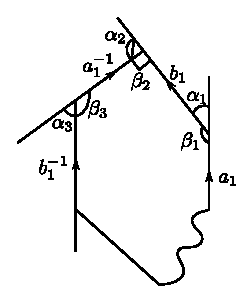
\includegraphics{vol9-figures/fig9-6.eps}}
  \end{figure}

2. ~ $D$ has elliptic varieties. 

Let the number of elliptic verities between $a_1$ and $b_1$ be $h_1$,  between
$a_2$ and $b_2$ be $h_2$, and so on. Here is included the case in
which some of the elliptic vertices are parabolic cusps. In this case
$(\pi - \beta_1 )$ must be replace by  
  \begin{figure}[H]
    \centerline{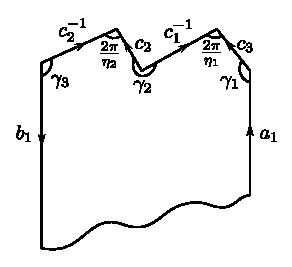
\includegraphics{vol9-figures/fig9-7.eps}}
  \end{figure}
\begin{gather*}
  (\pi - \gamma_1 ) + \left( \pi - \frac{2 \pi }{n_1}\right) + 
  (\pi - \gamma_2 ) + \left( \pi - \frac{2 \pi }{n_2}\right) +\cdots+ ( \pi -
  r _{h_1 + 1})\\ 
  = \pi - \sum_{ i = 1} ^{ h_1 + 1}\gamma_i + 2 \pi \sum_ { i = 1
  }^{ h_1  }  \left(1 - \frac{1}{n_i}\right) 
\end{gather*}\pageoriginale
where $n_1, \ldots $ are the orders of the substitutions leaving the
respective vertices fixed. In the case of a parabolic cusp, the angle
$\dfrac{2 \pi}{n_i}$ has to be replaced by $0$.  
  \begin{figure}[H]
    \centerline{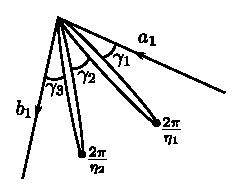
\includegraphics{vol9-figures/fig9-8.eps}}
  \end{figure}

We have therefore 
\begin{align*}
  \int \int\limits_D  d \omega & = \sum_{ h = h _1, h_2,\ldots} \left(\pi -
  \sum_{i = 1 }^{ h + 1} \gamma_i\right) + 2 \pi \sum_{\text{e.v.}} \left(1 -
  \frac{1}{n_1}\right) \\ 
  & = 4 \pi (g - 1) + 2 \pi \sum_{\text{e.v.}} \left(1 - \frac{1}{n_i}\right) 
\end{align*}
where e.v. stands for elliptic vertices including those which are
parabolic cusps in which case $\dfrac{1}{n_i}$ has to be replaced by
$0$. In the final form,  we obtain  
\begin{align*}
  \rho \iint \limits_D d \omega & = \rho \left\{ 4 \pi (g - 1) + 2 \pi
  \sum_{ e.  v.} \left(1- \frac{1}{n _i}\right)\right\} \\
  & = \prod_{ p | q_1} ( p - 1) \prod_{ p | q_2} (p + 1). 
\end{align*}

Since the constant $\rho$ is independent of the algebra, we can obtain
its value by considering the particular case where
$Q$ is a matrix algebra, $\mathcal{J} =  \begin{pmatrix}\mathscr{O} &
  \mathscr{O} \\ \mathscr{O} & \mathscr{O}\end{pmatrix}$, and then
$\mathscr{O}$ is the modular group. Here $q_1 = 1, q_2 = 1$and $D$ is
the fundamental domain for the modular group. The elliptic vertices
are $i$, $-\frac{1}{2} + \frac{\sqrt{3}}{2} i$, $\infty $  ($\infty $
begin a parabolic cup). The orders of the corresponding hyperbolic
motions are $2, 3, \infty $ respectively,  Further $ g = 0$,  since the
closed surface $s_{\mathcal{J}}$ is here the sphere. Hence we obtain  
$$
\rho \left\{ - 4 \pi + 2 \pi \left( 1- \frac{1}{2} + 1 - \frac{1}{3} + 1\right)
\right\} = 1, \text{ or } \rho = \frac{3}{\pi}. 
$$

Thus we arrive the complete formula 
$$
g = 1 - \frac{1}{2} \left( \sum_{\text{e.v.}} \left( 1 -
\frac{1}{n_i}\right)+ \sum_{ 
  \text{ parabolic cusps }}~  1 + \frac{1}{12}  \prod_{ p | q_1} ( p -
1)\prod_{ p | q_2} ( p+1)\right). 
$$
